\assignementTitle{}{26}{}

\putImgWOCaption{10cm}{1}

Требуется сконструировать и изготовить П-образную мостовую конструкцию (мостовой кран), 
по верхней перекладине которой перемещается каретка, а в нижней части (у основания опоры) 
расположен мотор. Вам необходимо разработать механизм линейного перемещения каретки и способ 
передачи движения от мотора к каретке. Требование, чтобы мотор находился внизу конструкции 
(а не непосредственно на каретке, например), может показаться не слишком обоснованным, 
но оно введено специально для усложнения задачи.

Каретка может иметь произвольную форму, но должна обеспечивать перемещение вдоль 
перекладины с минимумом качаний и люфтов. Размер поперечного сечения перекладины и 
опор не должен превышать 40х40 мм. Высота конструкции 150-300 мм, ширина (между опорами) - 
от 200 до 400 мм. Диапазон перемещения каретки должен составлять не менее $80\%$ расстояния между опорами.

В этом задании разрешается применить мотор любого типа, с любым способом управления 
(например, вручную переключателем), но лучше всего использовать шаговый двигатель, управляемый 
микроконтроллером.

Большая часть конструкции должна быть изготовлена с 
использованием технологий цифрового прототипирования (на ваш выбор и в соответствии 
с имеющимся оборудованием: 3D-печать, лазерная резка, фрезерование). Не разрешается использование 
конструктивных элементов из образовательных конструкторов (кроме мотора и шестерен, если требуется) или готовых узлов 3D-принтеров, но можно использовать трубки, профили, винтовые шпильки, ремни и т.п.  

Представляемые результаты:

\begin{enumerate}
    \item Сборочная модель конструкции, выполненная в любом САПР, с возможностью анимации
    \item Видеоролик или презентация, показывающая основные шаги изготовления конструкции (3D-печать, лазерная резка, фрезерование, сборка и пр.)
    \item Видеоролик, показывающий работу конструкции.
\end{enumerate}

При невозможности физически изготовить изделие, принимается анимированная сборочная модель 
(но, конечно, за нее начисляется меньше баллов). Учтите, что на очном туре команде все равно 
нужно как минимум уметь пользоваться 3D-принтером, а желательно еще и лазерным станком.

\solutionSection

Это конструкторское задание, и для него нет единственно правильного решения. Вот какие изделия представили некоторые из участников 2-го тура, прошедшие в финал:

\begin{tabular}{|p{7cm}|p{7cm}|}
    \hline
    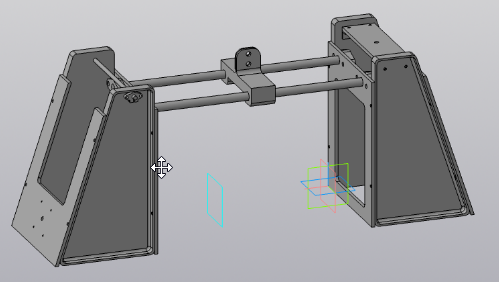
\includegraphics[width=7cm]{2} & 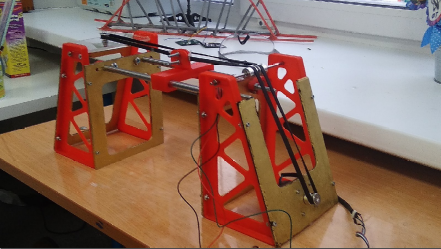
\includegraphics[width=7cm]{3} \\
    \hline
    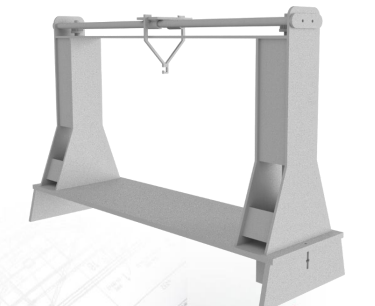
\includegraphics[width=7cm]{4} & 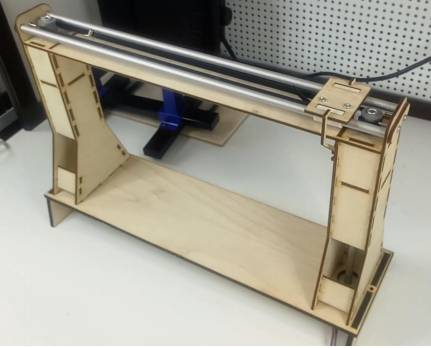
\includegraphics[width=7cm]{5} \\
    \hline
    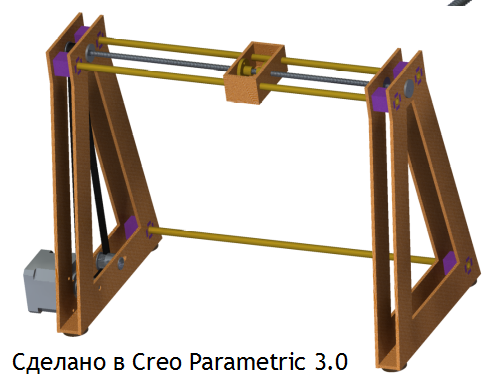
\includegraphics[width=7cm]{6} & 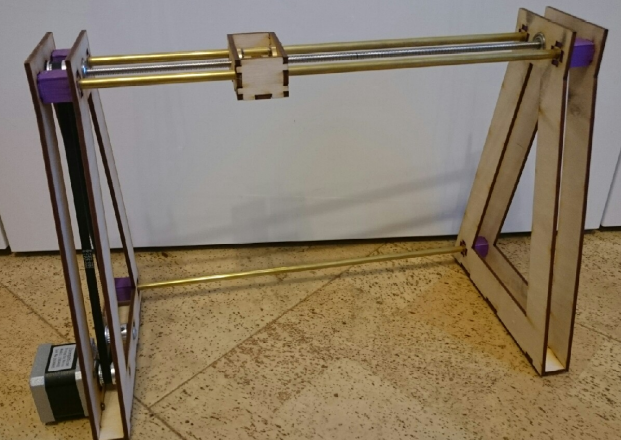
\includegraphics[width=7cm]{7} \\
    \hline
    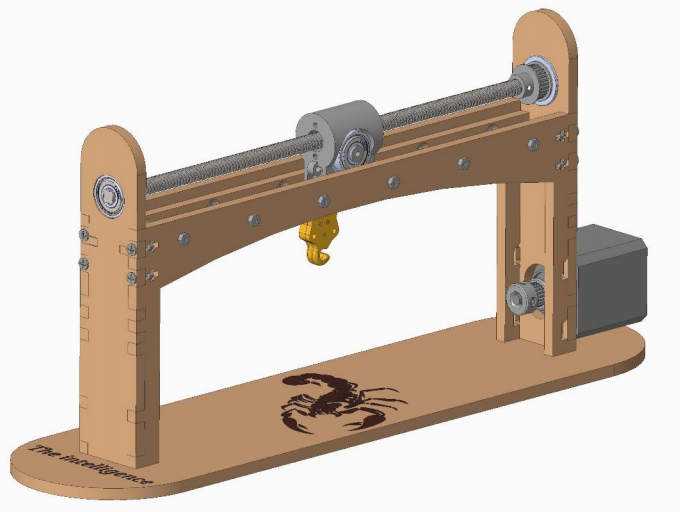
\includegraphics[width=7cm]{8} & 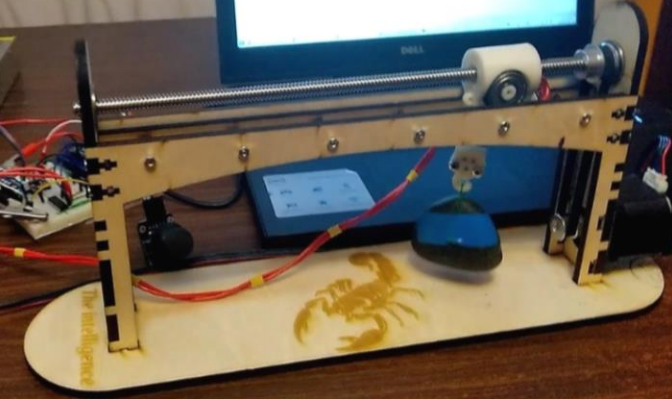
\includegraphics[width=7cm]{9} \\
    \hline
\end{tabular}